\documentclass[journal,10pt,twocolumn]{article}
\usepackage{graphicx}
\usepackage[margin=0.5in]{geometry}
\usepackage[cmex10]{amsmath}
\usepackage{array}
\usepackage{booktabs}
\usepackage{mathtools}
\title{\textbf{Conic section Assignment}}
\author{V.Meghana}
\date{October 2022}


\providecommand{\norm}[1]{\left\lVert#1\right\rVert}
\providecommand{\abs}[1]{\left\vert#1\right\vert}
\let\vec\mathbf
\newcommand{\myvec}[1]{\ensuremath{\begin{pmatrix}#1\end{pmatrix}}}
\newcommand{\mydet}[1]{\ensuremath{\begin{vmatrix}#1\end{vmatrix}}}
\providecommand{\brak}[1]{\ensuremath{\left(#1\right)}}
\providecommand{\lbrak}[1]{\ensuremath{\left(#1\right.}}
\providecommand{\rbrak}[1]{\ensuremath{\left.#1\right)}}
\providecommand{\sbrak}[1]{\ensuremath{{}\left[#1\right]}}

\begin{document}

\maketitle
\paragraph{\textit{Problem Statement} - Find the area of the region bounded by the curve $y^2=9x$ and the lines x=2 and x=4 and the axis in the first quadrant}

\section*{\large Solution}

\begin{figure}[h]
\centering
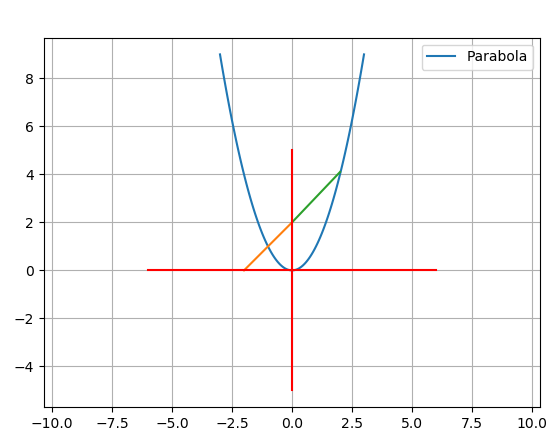
\includegraphics[width=1\columnwidth]{conics1.png}

\caption{The parabola formed by the curve $y^2 = 9x$ and the lines x=2 and x=4}
\label{fig:parabola}
\end{figure}

The given equation of parabola $y^2 = 9x$ can be written in the general quadratic form as
\begin{align}
    \label{eq:conic_quad_form}
    \vec{x}^{\top}\vec{V}\vec{x}+2\vec{u}^{\top}\vec{x}+f=0
    \end{align}
where
\begin{align}
 \label{eq:V_matrix}
 \vec{V} &= \myvec{0 & 0\\0 & 1},
 \\
 \label{eq:u_vector}
 \vec{u} &= \myvec{-4.5\\0},
 \\
 \label{eq:f_value}
 f &= 0
 %\\
\end{align}



The point of intersection of the lines x=2 and x=4 to the parabola is given by



The points of intersection of the line 
\begin{align}
 L: \quad \vec{x} = \vec{q} + \mu \vec{m} \quad \mu \in \mathbf{R}
\label{eq:conic_tangent}
\end{align}
with the conic section are given by
\begin{align}
\vec{x}_i = \vec{q} + \mu_i \vec{m}
\label{eq:conic_tangent_pts}
\end{align}
%
where
{\tiny
\begin{multline}
\mu_i = \frac{1}
{
\vec{m}^T\vec{V}\vec{m}
}
\lbrak{-\vec{m}^T\brak{\vec{V}\vec{q}+\vec{u}}}
\\
\pm
\rbrak{\sqrt{
\sbrak{
\vec{m}^T\brak{\vec{V}\vec{q}+\vec{u}}
}^2
-
\brak
{
\vec{q}^T\vec{V}\vec{q} + 2\vec{u}^T\vec{q} +f
}
\brak{\vec{m}^T\vec{V}\vec{m}}
}
}
\label{eq:tangent_roots}
\end{multline}
}



From the line x-2=0 the vectors q,m are taken,
\begin{equation}
\vec{q_2}=\myvec{2\\0}
\end{equation}

\begin{equation}
\vec{m_2}=\myvec{0\\1}
\end{equation}

by substituting eq(2),(3),(4),(8),(9) in eq(7)
\begin{equation}
\mu_i=\pm 3\sqrt{2}
\end{equation}
substituting eq(8),(9),(10) in eq(6) the intersection points on the parabola are
\begin{equation}
\vec{a_0}=\myvec{2\\3\sqrt{2}}
\end{equation}
\begin{equation}
\vec{a_1}=\myvec{2\\-3\sqrt{2}}
\end{equation}
From the line x-4=0 the vectors q,m are taken,
\begin{equation}
\vec{q_1}=\myvec{4\\0}
\end{equation}

\begin{equation}
\vec{m_1}=\myvec{0\\1}
\end{equation}

by substituting eq(2),(3),(4),(13),(14) in eq(7)
\begin{equation}
\mu_i=\pm 6
\end{equation}
substituting eq(13),(14),(15) in eq(6) the intersection points on the parabola are
\begin{equation}
\vec{a_3}=\myvec{4\\6}
\end{equation}
\begin{equation}
\vec{a_2}=\myvec{4\\-6}
\end{equation}

Area of the parabola in between the lines x=2 and x=4 is given by
\begin{align}
\implies A_1=\int_{0}^{2} \ 3\sqrt{x} \,dx
\end{align}

\begin{align}
\implies A_2=\int_{0}^{4} \ 3\sqrt{x} \,dx
\end{align}
\begin{align}
\implies A_2- A_1=\int_{0}^{4} \ 3\sqrt{x} \,dx-\int_{0}^{2} \ 3\sqrt{x} \,dx
\end{align}
\begin{align}
\implies A_2- A_1=16-4\sqrt{2}
\end{align}


\section*{\large Construction}

{
\setlength\extrarowheight{5pt}
\begin{tabular}{|l|c|}
    \hline 
    \textbf{Points} & \textbf{intersection points} \\ \hline
   a0 & $\myvec{
   2\\
   3\sqrt{2}
   } $ \\\hline
   a1 & $\myvec{
   2\\
   -3\sqrt{2}
   } $ \\\hline
    
   a3 & $\myvec{
   4\\
   6
   } $ \\\hline
   a2 & $\myvec{
   4\\
   -6
   } $ \\\hline
      
      \end{tabular}
}

\end{document}
